\begin{frame}{Biomas}
    \begin{itemize} \setlength\itemsep{1em}
        \item Neste trabalho biomas são características de relevo;
        \item Foram implementados cinco biomas distintos;
        \item Suas características de cor e cálculo de altura foram escolhidos arbitrariamente
        para serem distitos.
    \end{itemize}
    
%    \begin{figure}
%        \centering
%        \begin{subfigure}[b]{0.47\textwidth}
%            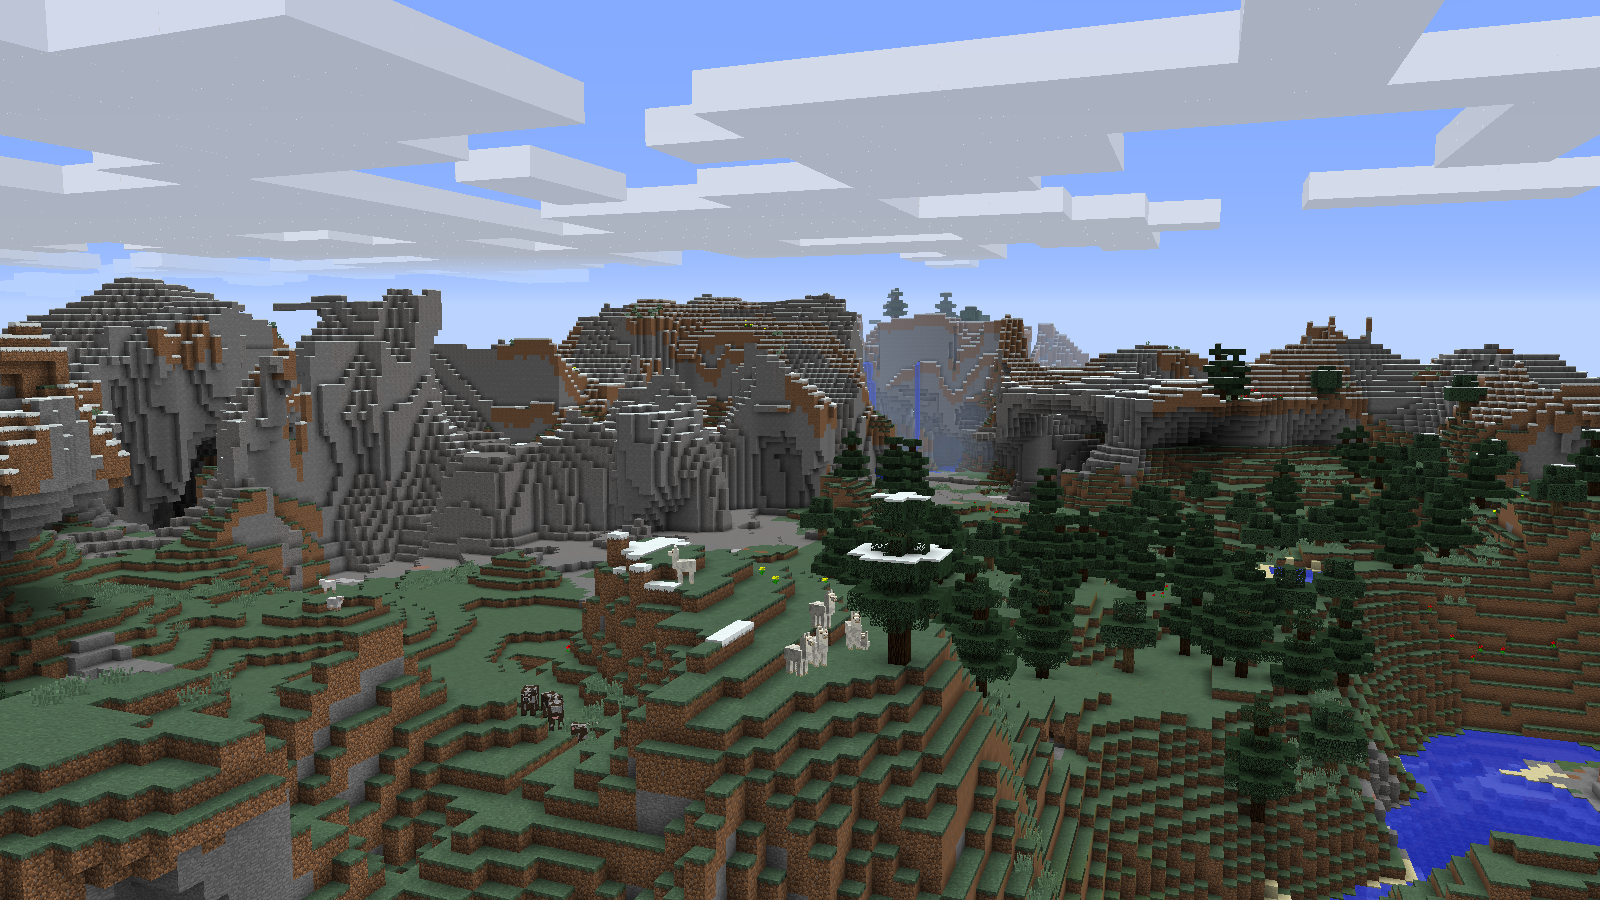
\includegraphics[width=\textwidth]{img/mineExtremeHills}
%            \caption{Bioma \textit{Extreme Hills} no minecraft}
%            \label{fig:mineExtremeHills}
%        \end{subfigure}
%        ~ %add desired spacing between images, e. g. ~, \quad, \qquad, \hfill etc. 
%          %(or a blank line to force the subfigure onto a new line)
%        \begin{subfigure}[b]{0.47\textwidth}
%            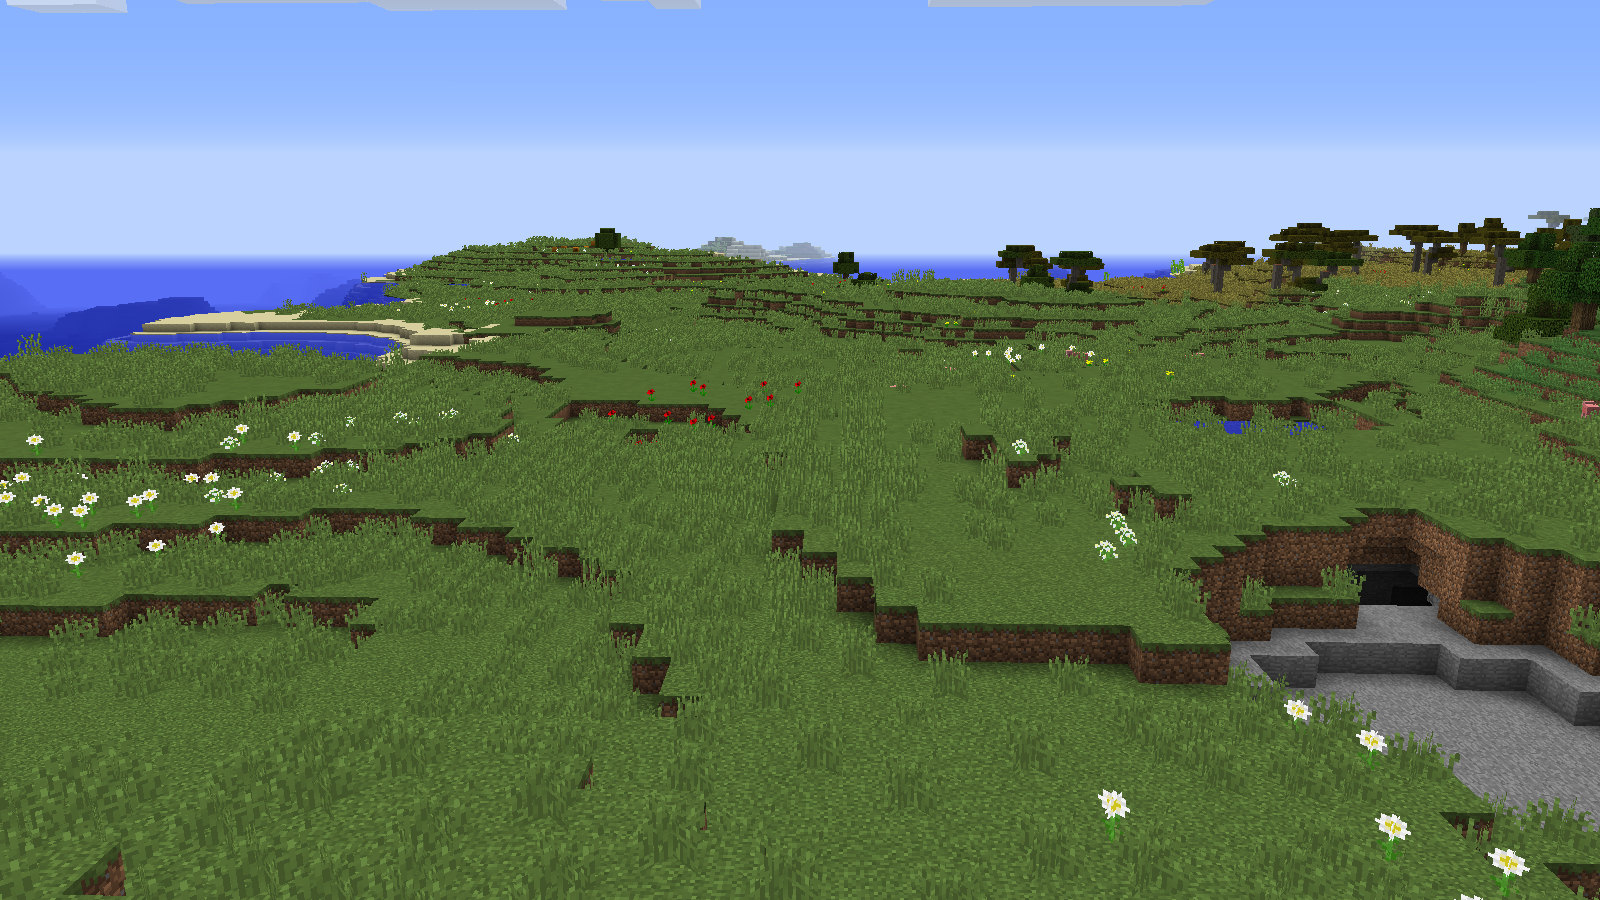
\includegraphics[width=\textwidth]{img/minePlains}
%            \caption{Bioma \textit{Plains} no minecraft}
%            \label{fig:minePlains}
%        \end{subfigure}
%        ~ %add desired spacing between images, e. g. ~, \quad, \qquad, \hfill etc. 
%        %(or a blank line to force the subfigure onto a new line)
%        \caption{Exemplo de Biomas no minecraft}
%        \label{fig:mineBiomes}
%    \end{figure}
    
    
\end{frame}

\begin{frame}{Biomas}
    \begin{figure}[H]
        \centering
        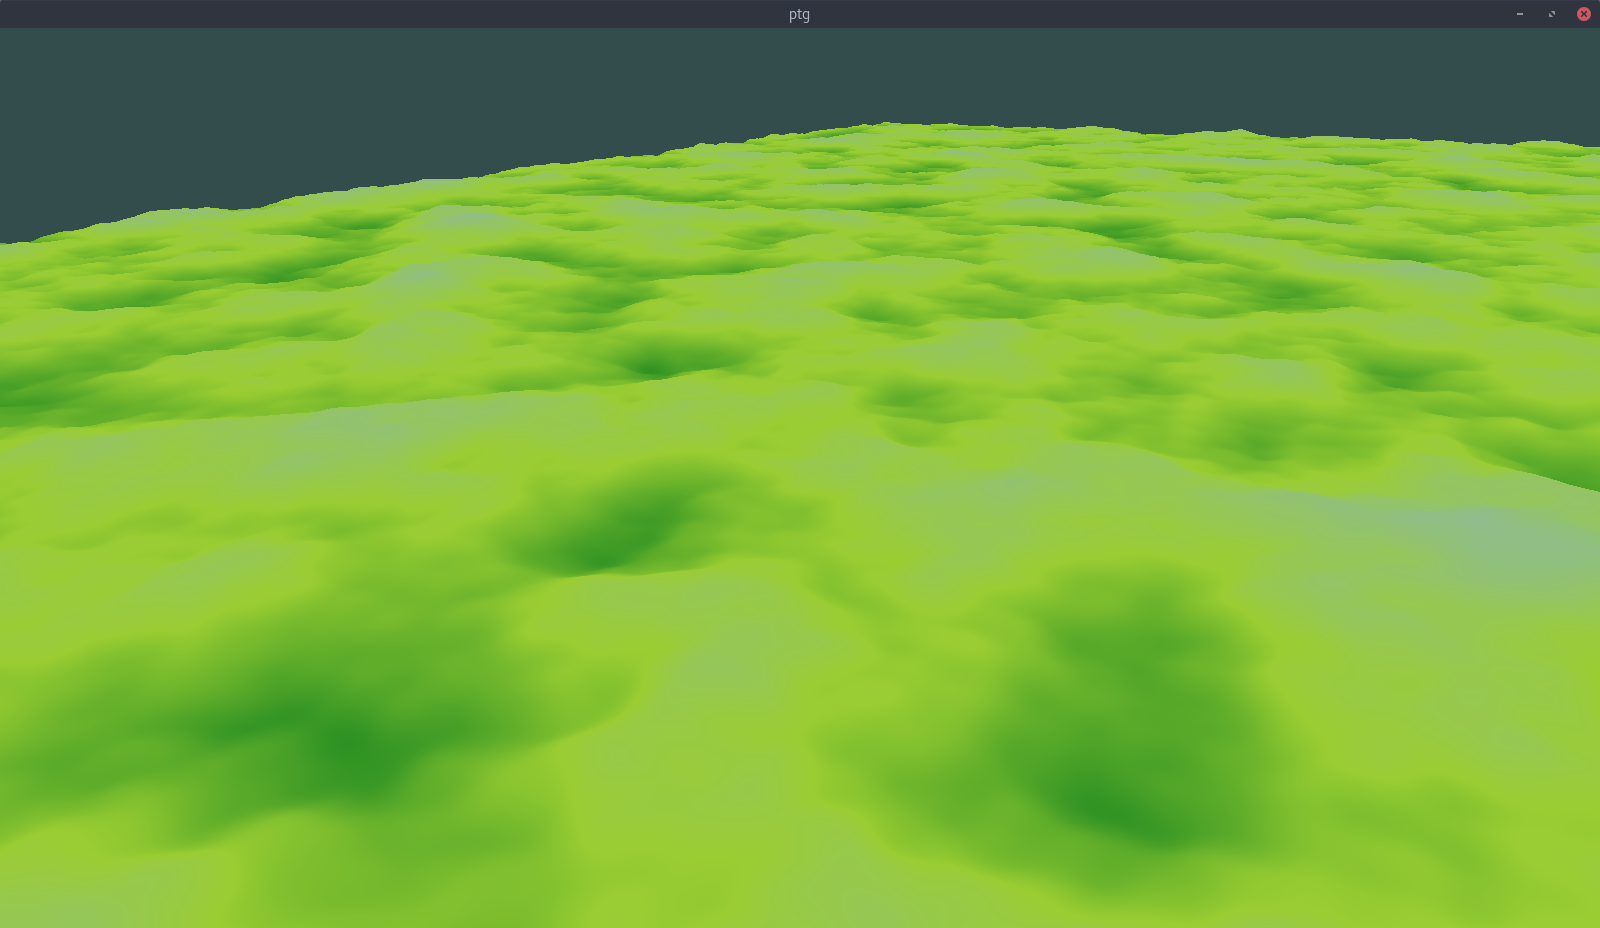
\includegraphics[width=.9\textwidth]{img/biomas/bssPlains.png}
        \caption{Bioma: Planícies.}
        \label{fig:img_biomas_bssPlains}
    \end{figure}
    
    
\end{frame}

\begin{frame}{Biomas}
    \begin{figure}[H]
        \centering
        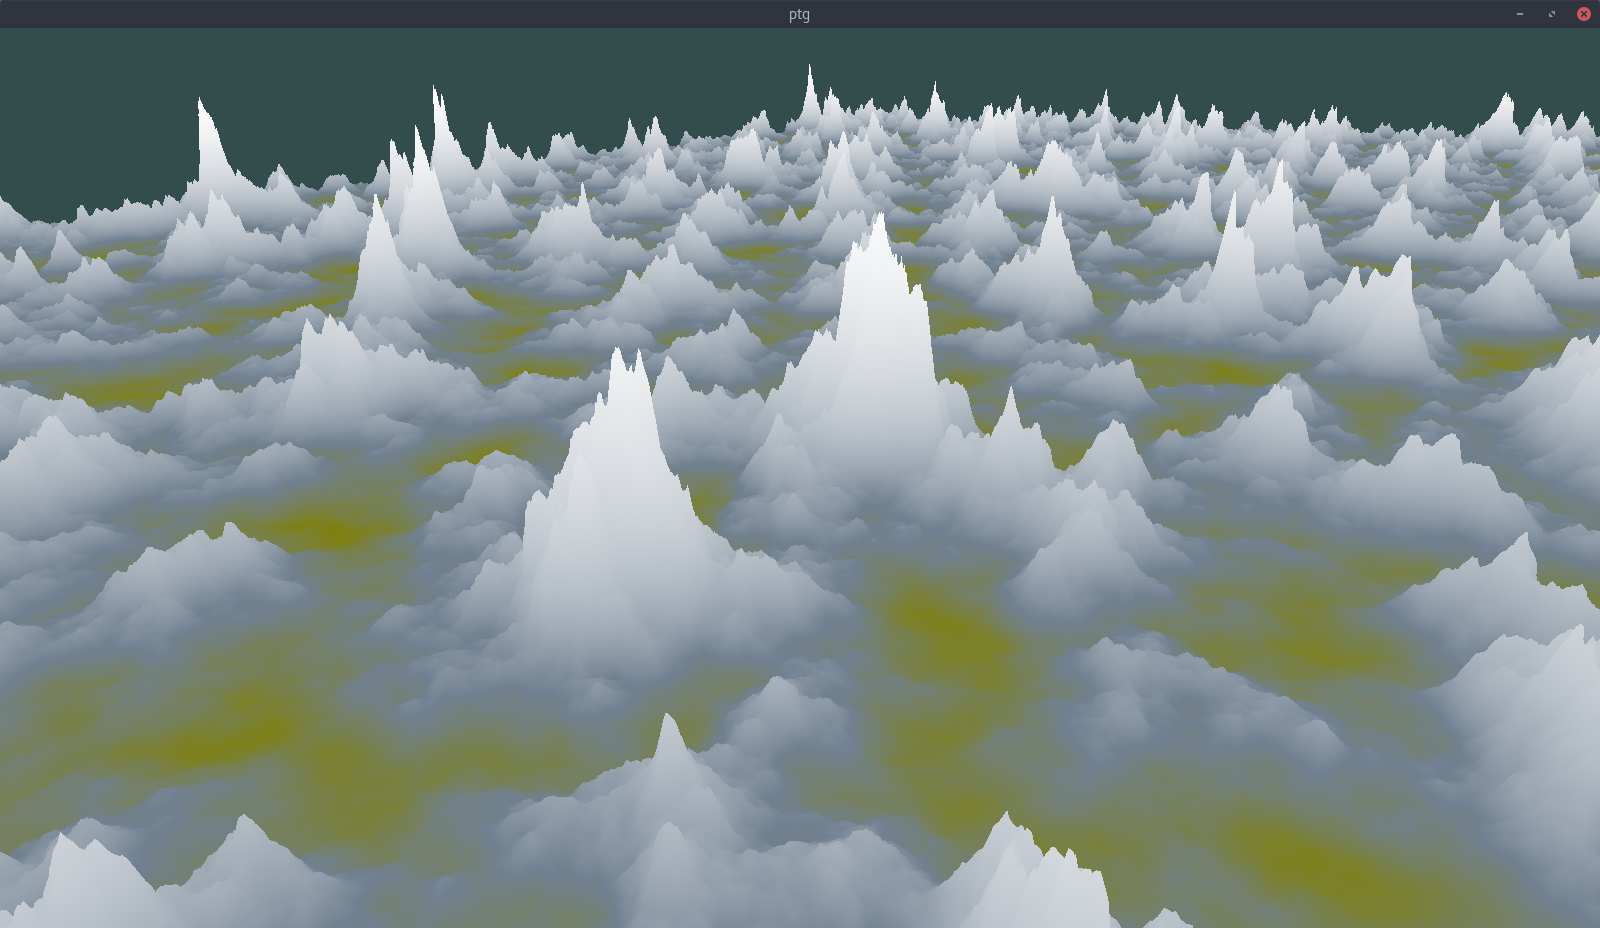
\includegraphics[width=.9\textwidth]{img/biomas/bssMontains.png}
        \caption{Bioma: Montanhas.}
        \label{fig:img_biomas_bssMontains}
    \end{figure}
    
    
\end{frame}

\begin{frame}{Biomas}
    \begin{figure}[H]
        \centering
        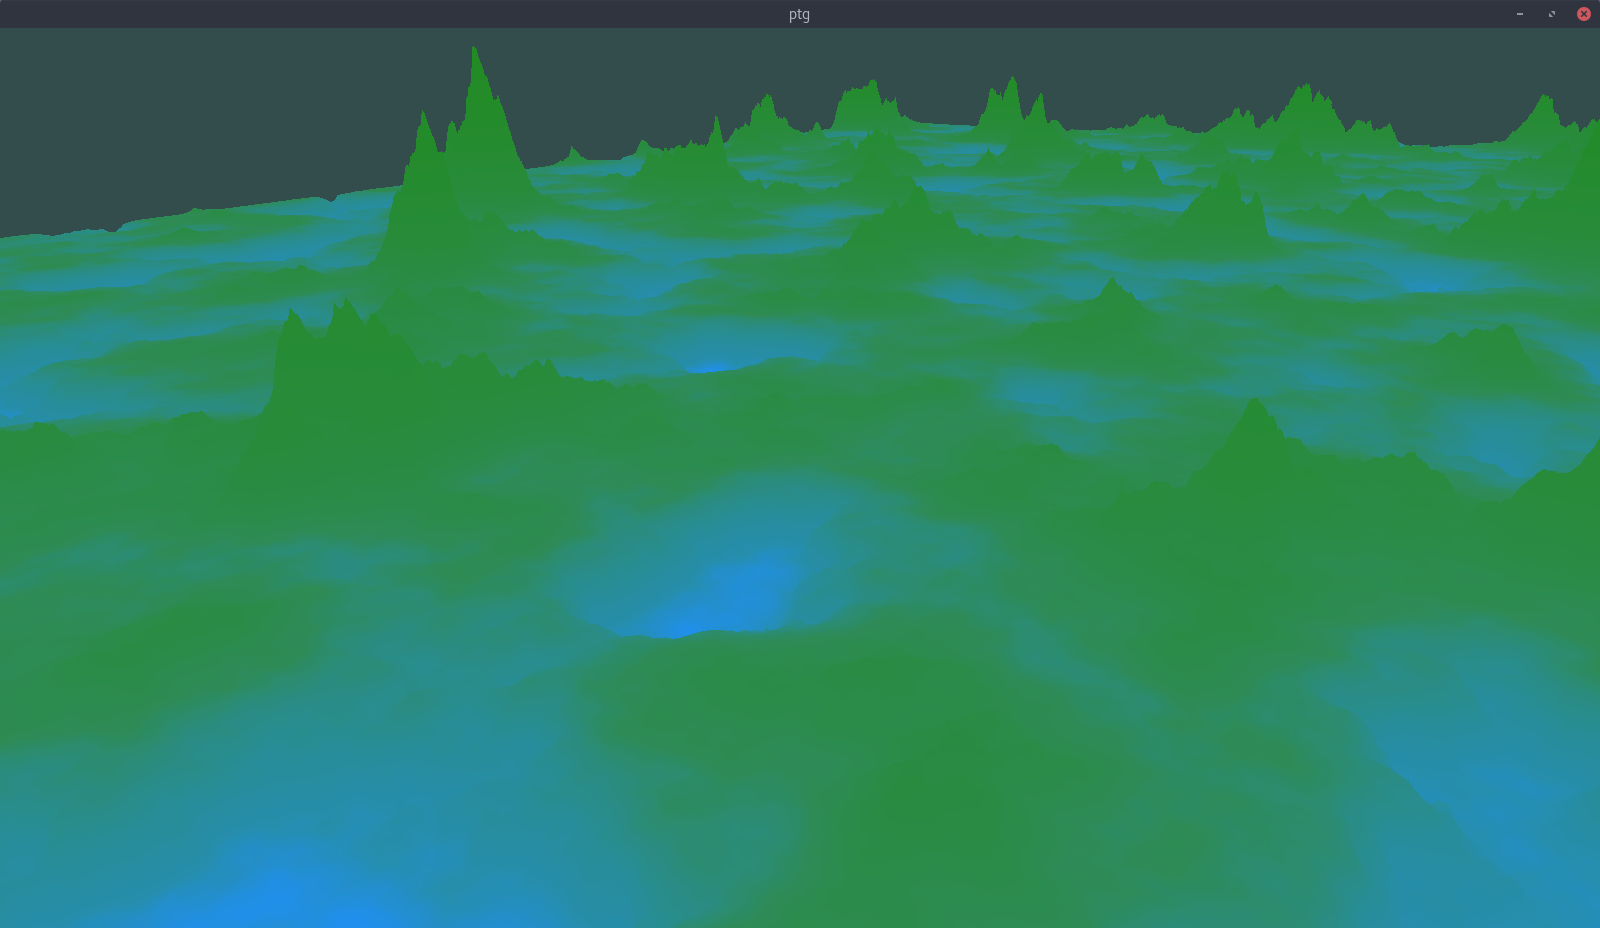
\includegraphics[width=.9\textwidth]{img/biomas/bssValley.png}
        \caption{Bioma: Vales.}
        \label{fig:img_biomas_bssValley}
    \end{figure}
    
    
\end{frame}

\begin{frame}{Biomas}
    \begin{figure}[H]
        \centering
        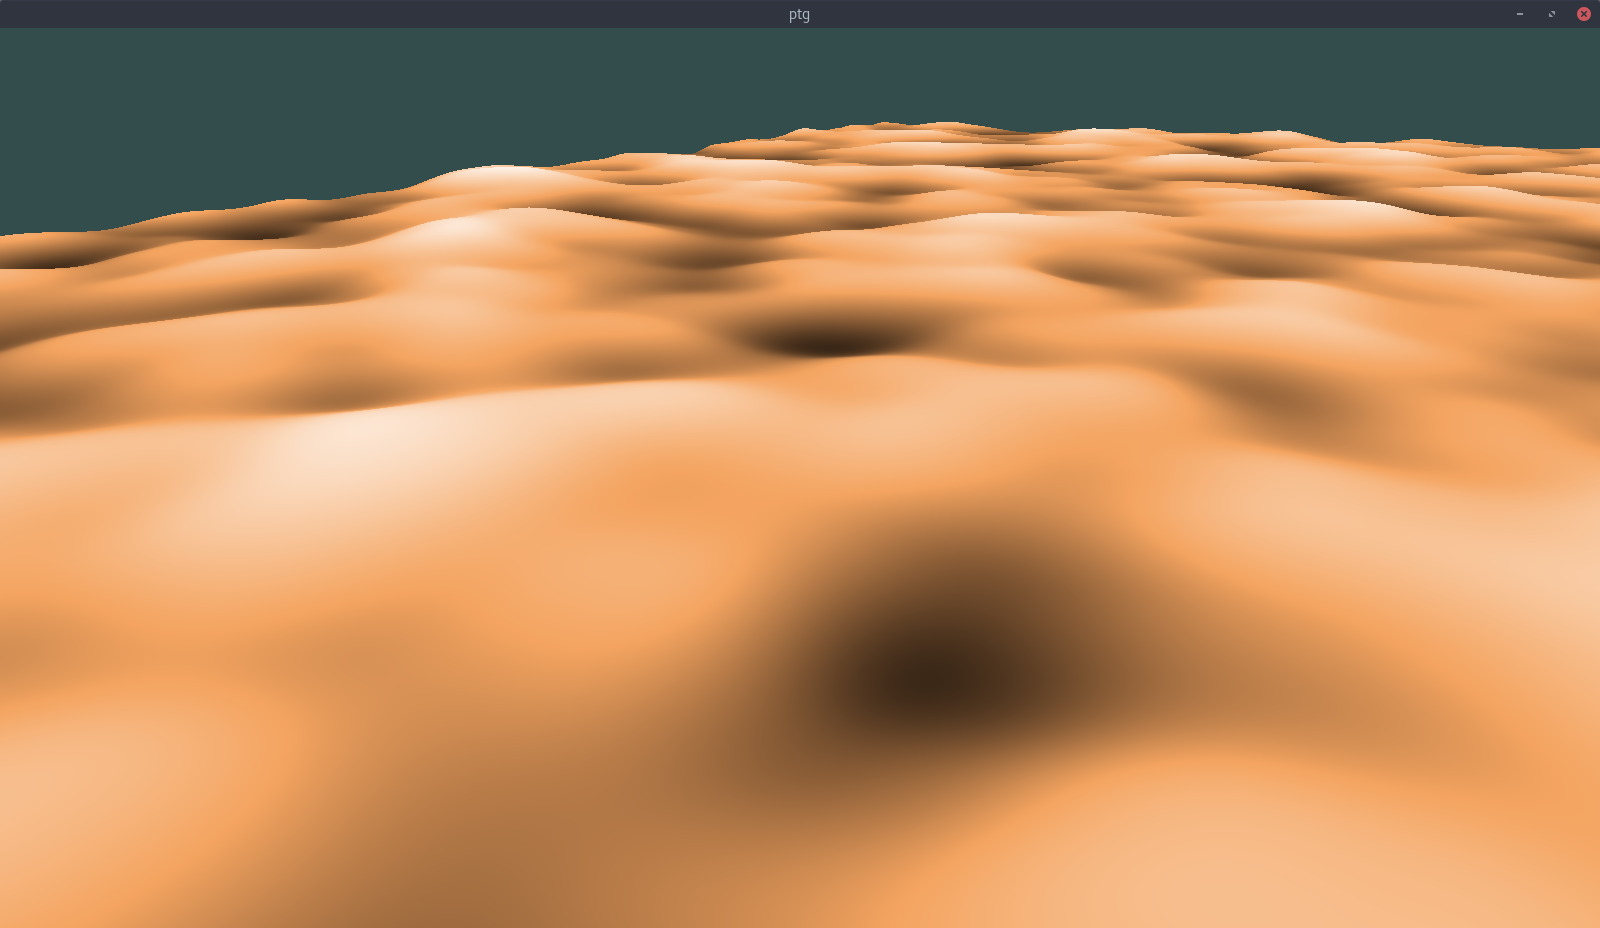
\includegraphics[width=.9\textwidth]{img/biomas/bssDesert.png}
        \caption{Bioma: Deserto.}
        \label{fig:img_biomas_bssDesert}
    \end{figure}
    
    
\end{frame}

\begin{frame}{Biomas}
    \begin{figure}[H]
        \centering
        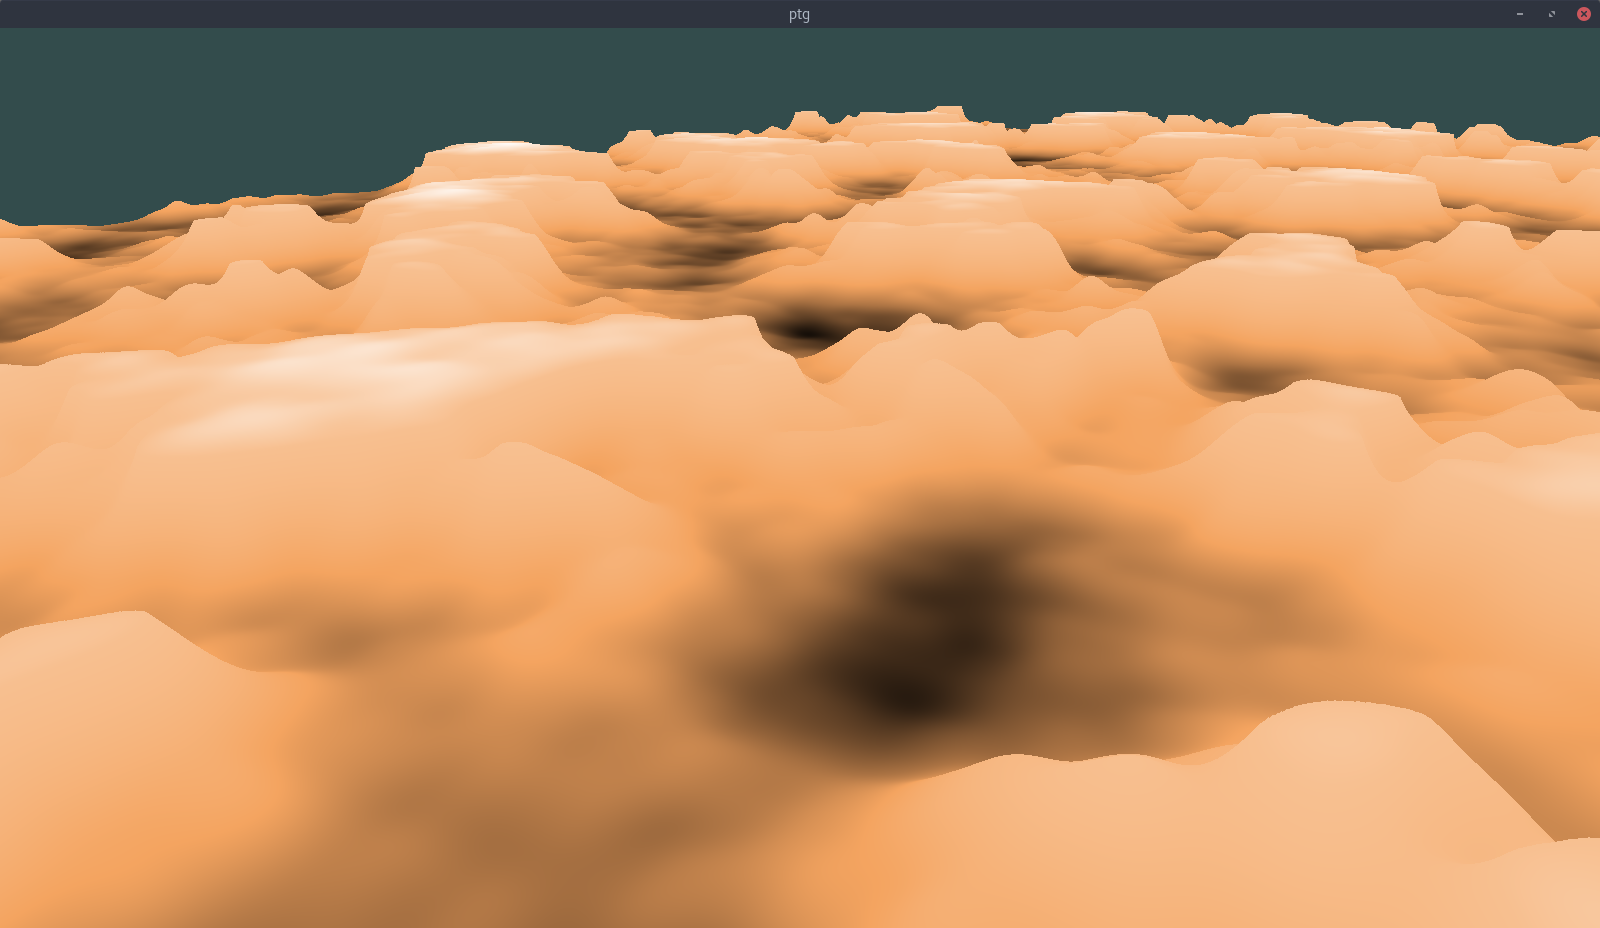
\includegraphics[width=.9\textwidth]{img/biomas/bssCanyons.png}
        \caption{Bioma: Cânyons.}
        \label{fig:img_biomas_bssCanyons}
    \end{figure}
    
    
\end{frame}